\documentclass{article}
\usepackage{graphicx}

\begin{document}
	
	\begin{table}[h!]
		\centering
		\caption{Heart Disease Data}
		\label{tb}
		\begin{tabular}{|l|l|l|l|l|l|l|l|l|l|l|l|l|l|}
			\hline
			age & sex & cp & trestbps & chol & fbs & restecg & thalach & exang & oldpeak & slope & ca & thal & target \\ \hline
			63 & 1 & 3 & 145 & 233 & 1 & 0 & 150 & 0 & 2.3 & 0  & 0 & 1 & 1 \\ \hline
			37 & 1 & 2 & 130 & 250 & 0 & 1 & 187 & 0 & 3.5 & 0  & 0 & 2 & 1 \\ \hline
			41 & 0 & 1 & 130 & 204 & 0 & 0 & 172 & 0 & 1.4 & 2  & 0 & 2 & 1 \\ \hline
			56 & 1 & 1 & 120 & 236 & 0 & 1 & 178 & 0 & 0.8 & 2  & 0 & 2 & 1 \\ \hline
			57 & 0 & 0 & 120 & 354 & 0 & 1 & 163 & 1 & 0.6 & 2  & 0 & 2 & 1 \\ \hline
			57 & 1 & 0 & 140 & 192 & 0 & 1 & 148 & 0 & 0.4 & 1  & 0 & 1 & 1 \\ \hline
			56 & 0 & 1 & 140 & 294 & 0 & 0 & 153 & 0 & 1.3 & 1  & 0 & 2 & 1 \\ \hline
			44 & 1 & 1 & 120 & 263 & 0 & 1 & 173 & 0 & 0 & 2  & 0 & 3 & 1 \\ \hline
			% Add more rows as needed


\end{tabular}

\end{table}

	
	\begin{figure}
			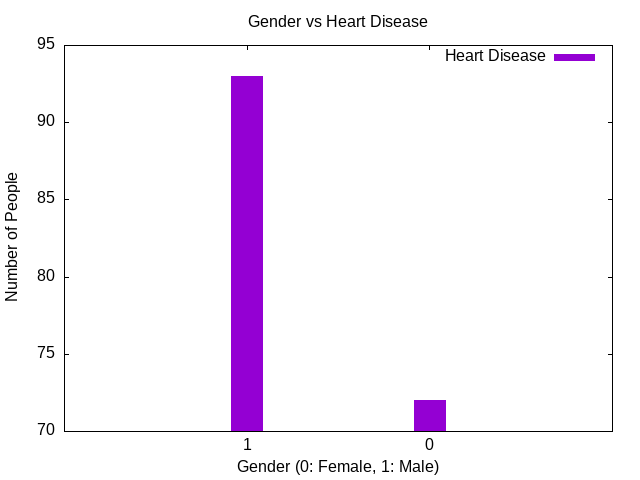
\includegraphics[width=\textwidth]{gender_vs_heart_disease.png}
		\caption{Histogram plot between gender and heart diseases}
		\label{f1}
	\end{figure}

\begin{figure}
	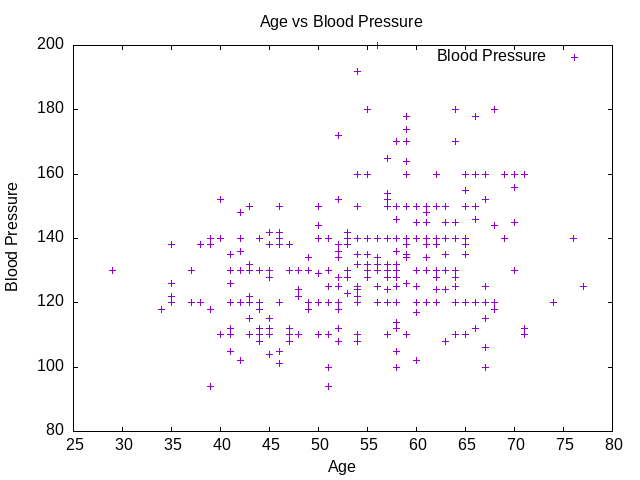
\includegraphics[width=\textwidth]{age_vs_blood_pressure.png}
	\caption{Scattered plot between age and blood pressure}
	\label{f2}
\end{figure}
 
 \begin{figure}
 	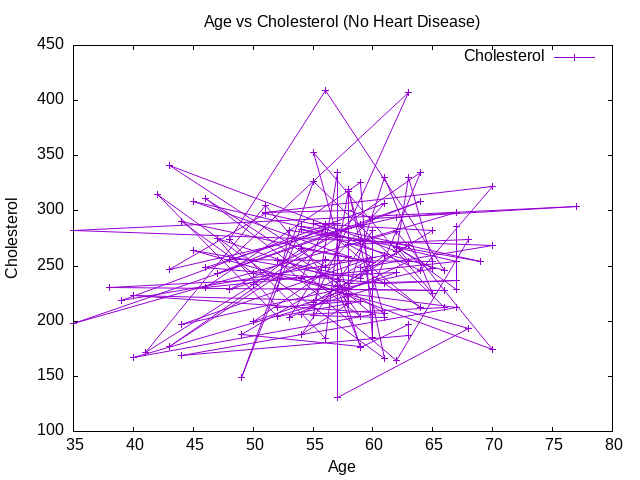
\includegraphics[width=\textwidth]{age_vs_chol_no_disease.png}
 	\caption{Line plot between age and cholestrol}
 	\label{f3}
 \end{figure}

	
		
	 Above we have four plots in reference to table ~\ref{tb}: Fig ~\ref{f1}. Showing hiostogram plot between gender and heart diseases, Fig ~\ref{f2} Showing scattered plot between age and blood pressure , fig~\ref{f3} showing lineplot between age and cholestrol andFig~\ref{f4}showing piechart between age groups and heart diseases.


\end{document}
